
Auf Basis der in der Balkenberechnung bestimmten Parameter Biegesteifigkeit, maximales Biegemoment und der maximalen Querkraft, sollen die Gurte und der Steg dimensioniert werden. Die Vorauslegung soll dabei anhand der VDI-Richtlinie 2013 erfolgen, diese enthält in einem Unterkapitel Informationen speziell zur Auslegung eines I-Trägers. Dabei ist zu beachten, dass für die Auslegung vorgeschlagene Kennwerte verwendet werden, die im Allgemeinen nicht exakt den tatsächlichen Materialkennwerten des gewählten Verbundes entsprechen. Zusätzlich sei angemerkt, dass die erste Auslegung nur an ausgewählten Stellen Sicherheitsfaktoren ungleich eins berücksichtigt. Grund dafür ist die Annahme, dass in den bereitgestellten Materialkennwerten ausreichende Sicherheiten verrechnet worden sind. Die grobe Vorauslegung hat den Anspruch die Grundlage für die aufbauende Berechnung mithilfe eines Laminatrechners zu legen.

\subsection{Dimensionierung der Gurte mit rechteckigem Querschnitt}
\label{GurtDim}
Bei der Auslegung der Gurte auf Steifigkeit wird angenommen, dass der Steg des I-Trägers keine Längskräfte aufnimmt und der Biegung nicht entgegenwirken kann. Die in der Balkenberechnung ermittelte Biegesteifigkeit $ EI_{x} = 962,31 Nm^{2} $, die erforderlich ist, damit bei einer Kraft $ F_{pruef}=100N $ die Flügelspitze eine Absenkung von $ w_{j=1,1}=20mm $ erfährt, muss allein durch die Gurte aufgebracht werden. Im Sinne der kraftflussgerechten Gestaltung sollen die Glasfasern unidirektional in Längsrichtung des Gurtes angeordnet werden. Die Bezeichnungen der Längenangaben des Holmes orientieren sich an Abb.~\ref{fig: Rechteckholm}~.\\

\begin{figure}[h]
	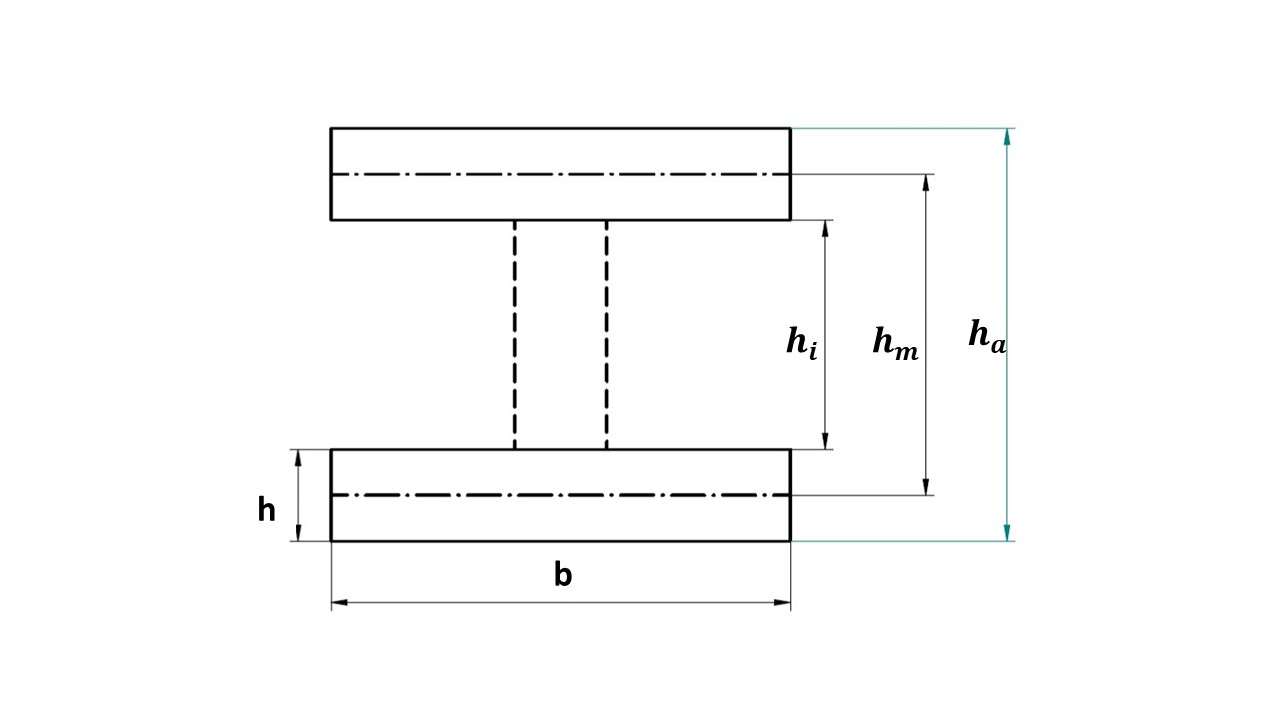
\includegraphics[width=1.0\textwidth]{Bilder/RechteckHolm.jpg}
	\caption{Bezeichnungen des I-Holms}
	\label{fig: Rechteckholm}
\end{figure}

\noindent Die Gurte werden zur Bestimmung der notwendigen Lagenanzahl als rechteckig angenommen, erst in einem späteren Schritt soll die Form der Kontur der vorgegebenen Haut angepasst werden. Die Maße sind über die gesamte Länge des Holms als konstant anzusehen.\\
Zur Bestimmung des Flächenträgheitsmomentes $ I_{x} $ wird der E-Modul in Längsrichtung der Fasern nach der Mischungsregel gemäß [3] berechnet.\\
\begin{equation}
 E_{11}=  \varphi\cdot E_{f,11}+\left( 1-\varphi \right) \cdot E_{M}
\end{equation}
Mit den gegebenen Materialkennwerten $ E_{f,11}=74000MPa $, $ E_{m}=3300MPa $ und $ \varphi=0,4 $ bestimmt sich $ E_{11} = 31580 MPa $. Damit ergibt sich ein benötigtes Flächenträgheitsmoment von 
\begin{equation}
	I_{x,min} = \frac{962,31Nm^{2}}{31580\cdot 10^{6}Pa} =3,04722 \cdot 10^{-8} m^{4}
\end{equation}

\noindent Das Flächenträgheitsmoment der Gurte bestimmt sich aus den Flächenträgheitsmomenten der beiden Rechteckquerschnitte und ihren zugehörigen Steiner-Anteilen, die aus der Verschiebung der Gurte um jeweils $ \frac{h_{m}}{2} $ in z-Richtung resultieren.
\begin{equation}
	\label{Ix}
	I_{x}=2\cdot\left(\frac{b\cdot h^{3}}{12}+b\cdot h\cdot\left(\frac{h_{m}}{2}\right)^{2}\right)
\end{equation}

\noindent Es wird nach einer Kombination aus Gurtbreite $ b $ und Gurthöhe $ h $ gesucht, die die Anforderungen an das Flächenträgheitsmoment erfüllt, aber dennoch zu einer möglichst geringen Gurtquerschnittsfläche und damit zu einer möglichst geringen Masse der Gurte führt. Um die Steiner-Anteile der Gurte zu maximieren, sollen die Gurte in einem möglichst großen Abstand zur neutralen Faser angeordnet werden. Vorgegeben ist eine Profildicke von $ 37,5mm $, allerdings muss berücksichtigt werden, dass die nach innen gelegte Haut, die Wölbungsrücklage und die Dickenrücklage die maximale Höhe des Holmes einschränken. Deshalb wird die gesamte Gurthöhe auf $ h_{a}=36mm $ abgeschätzt. Die dadurch begrenzte Anzahl der Lagen in der Haut wird im Abschnitt "CAD-Modell" weiter erläutert.\\ 

\noindent Tabelle ~\ref{bh} enthält Werte der Gurtquerschnittsfläche bei verschiedenen Kombinationen von $ b $ und $ h $, die zum erforderlichen gesamten Flächenträgheitsmoment von $ I_{x,min} = 3,04722 \cdot 10^{-8} m^{4} $ führen.\\
\begin{table}[h]
	\caption{Verschiedene Kombinationsmöglichkeiten von $ b $ und $ h $}
	\label{bh}
	\begin{center}
		\begin{tabular}{l|c|r}
			$h$&$b$&$2\cdot b\cdot h$\\
			\hline
			$1mm$&$38,3mm$&$76,6mm^{2}$\\
			$1,25mm$&$31,1mm$&$77,7mm^{2}$\\
			$1,5mm$&$26,3mm$&$78,8mm^{2}$\\
			$2,25mm$&$18,3mm$&$82,3mm^{2}$\\
		\end{tabular}
	\end{center}
\end{table}

\noindent Den Daten ist zu entnehmen, dass breite Gurte geringer Dicke bei gleichem Flächenträgheitsmoment geringere Querschnittsflächen aufweisen. Aus diesem Grund sollen die Gurte möglichst breit gewählt werden. Die Breite der Gurte ist durch die vorgegebene Konstruktion der Platte zur Aufnahme der Tragfläche am Teststand begrenzt. Die vorgesehene Aussparung weist eine Breite von $ 30mm $ auf. Für die weitere Berechnung soll $ b=28mm $ gelten. Diese Annahme wird dadurch begründet, dass die Fertigung des Holms im Bereich des Modellbaus von Hand erfolgen würde, womit nur grobe Toleranzen einhaltbar sind.\\

\noindent Mithilfe eines Solvers bestimmt sich aus dem Flächenträgheitsmoment und der Gurtbreite die Gurthöhe $ h=1,866mm $.\\
\noindent Im nächsten Schritt wird die zu stapelnde Lagenanzahl ermittelt. Als vorwiegend unidirektionales Material steht das Glasgewebe Interglas 92145 mit einem Flächengewicht von $ 220\frac{g}{m^{2}} $ zur Verfügung. Nach \cite{item3} berechnet sich die Lagenanzahl $ n $ für eine Dicke des Verbundes $ t_{soll} $ zu:\\

\begin{equation}
	\label{gurtlagen}
	n=t_{soll}\cdot \frac{\varphi\cdot\rho_{f}}{\left(\frac{m_{f}}{L\cdot b}\right)}
\end{equation}

\noindent Mit $ \left(\frac{m_{f}}{L\cdot b}\right) = 220\frac{g}{m^{2}} $, $ t_{soll}=h $ und $ \rho_{f}=2550\frac{kg}{m^{3}} $ ergibt sich $ n=8,653 $. Es sind also 9 Lagen des Gewebes 92145 für jeden Gurt vorzusehen.Die sich aus 9 Lagen ergebende Gurthöhe kann durch Umstellen von Gleichung ~\ref{gurtlagen} zu $ \tilde{h}=1,941mm $ bestimmt werden. Für den zunächst angenommenen Fall von Gurten mit rechteckigen Querschnitten ist die Auslegung zur Einhaltung der Anforderungen an die Steifigkeit damit abgeschlossen.\\


\subsection{Nachrechnung der angepassten Gurte}
 Die Modellierung der Haut und der Holmgurte in einem CAD-Programm zeigt, dass die Gurte mit den berechneten Bemaßungen nicht innerhalb des Profils mit der als $ 0,75mm $ dick angenommenen Haut liegen. Die Anpassung der Konstruktion der Gurte erfolgt so, dass die Gurtoberseite an der Innenseite der Haut anliegt.Die Gesamtbreite von $ 28mm $, sowie die Gurtdicke $ h $ bleiben dabei erhalten. Die Gesamthöhe $ h_{a} $ muss auf $ \tilde{h_{a}}=35,8mm $ leicht verringert werden. Abbildung ~\ref{fig: KrummerGurt} veranschaulicht die gekrümmte Form des oberen Holmgurtes.
 \begin{figure}[h]
 	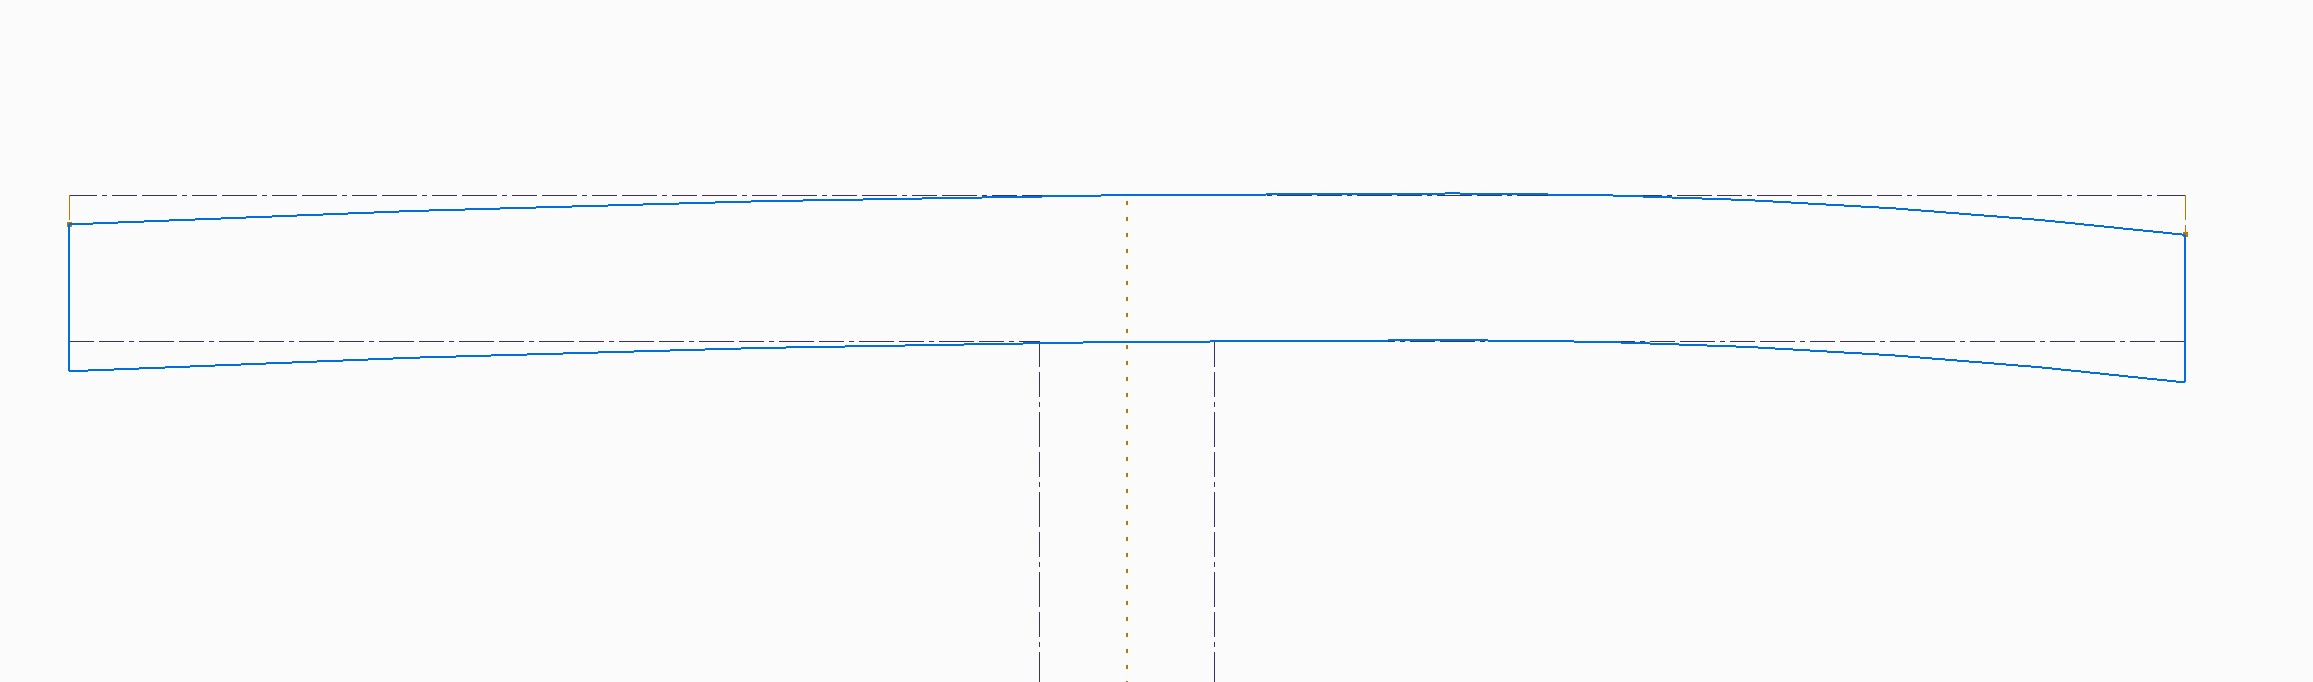
\includegraphics[width=1.0\textwidth]{Bilder/KrummerGurt.jpg}
 	\caption{Angepasste gekrümmte Gurtkontur}
 	\label{fig: KrummerGurt}
 \end{figure}

\noindent Die angepasste Krümmung der Gurte führt zu einem veränderten Flächenträgheitsmoment $ \tilde{I_{x}} $ des Balkens, dass mithilfe des CAD-Programms exakt zu $ \tilde{I_{x}}=3,075406\cdot 10^{-8}m^{4} $ bestimmt werden kann. Da 
\begin{equation}
	\label{IVergleich}
	\tilde{I_{x}}=3,075406\cdot 10^{-8}m^{4} > I_{x,min}=3,04722\cdot 10^{-8}m^{4}
\end{equation}
gilt, genügen auch die veränderten Gurte der Steifigkeitsanforderung.\\
 
\noindent Abschließend wird gezeigt, dass die Festigkeit der Gurte einer Belastung der Flügelspitze durch $ F_{pruef}=500N $ standhält. Die aus der Biegung resultierenden und betragsmäßig gleichen Zug- und Druckspannungen werden dazu mit den vorhandenen UD-Festigkeitskennwerten des Handlaminats verglichen. Die Resultate der Balkenberechnungen zeigen, dass das maximale Biegemoment im Holm an Punkt C auftritt und $ M_{b}=500N\cdot 0,773m=386,5Nm $ beträgt.In den Randfasern der Gurte resultieren Spannungen, die sich nach\\
\begin{equation}
	\sigma_{b}=\frac{M_{b}\cdot \tilde{h_{a}}}{\tilde{I_{x}}\cdot 2}
\end{equation} 
zu $ \sigma_{b}=224,96MPa $ berechnen. Da 
\begin{equation}
	\sigma_{b}< R^{(+)}_{||}=597,9 MPa < |R^{(-)}_{||}| =650,0 MPa
\end{equation} 
gilt, ist der Festigkeitsnachweis erbracht. Es kann davon ausgegangen werden, dass die Gurte bei einer Prüfkraft von $ F_{pruef}=500N $ nicht versagen. \\

\subsection{Bestimmung der Lagenanzahl des Steges}
Die Auslegung des Steges erfolgt auch anhand der VDI 2013. Dabei muss beachtet werden, dass der Steg sowohl durch Schubkräfte als auch durch Normalkräfte senkrecht und parallel zu den Gurten Belastungen erfährt. Die Dehnungen der Innenseiten der Gurte werden dem Steg aufgeprägt, da beide Bauteile stoffschlüssig miteinander verbunden sind. Anders als in der VDI 2013 wird jedoch nicht die Bruchdehnung der Gurte betrachtet, sondern die Dehnungen der Innenseiten bei einer Prüfkraft von 500N. So soll die Dimensionierung des Steges auf die Anforderungen an die Festigkeit angepasst werden, um Leichtbaupotentiale bestmöglich auszuschöpfen.\\

\noindent Die größte Längsdehnung der Gurte tritt an der Stelle C auf, da dort das größte Biegemoment wirkt. Sie lässt sich für die Innenseite der Gurte durch
\begin{equation}
	\epsilon_{Gurt}=\frac{\sigma_{innen}}{E_{11}}=\frac{\frac{F_{pruef}\cdot l_{3}\cdot h_{i}}{\tilde{I}_{x}\cdot 2}}{E_{11}}
\end{equation}  
 zu $ \epsilon_{Gurt}=6,351\cdot 10^{-3} $ berechnen. Auf der Zugseite ist die Dehnung positiv, auf der Druckseite negativ. Die dem Steg aufgeprägte Dehnung führt in Längsrichtung des Steges zu einem Normalkraftfluss, der sich nach VDI 2013 mit
 \begin{equation}
 	p_{\epsilon}=n\cdot \bar{q}\cdot K_{E\#}\cdot \epsilon_{Gurt}
 \end{equation} 
ermitteln lässt. $ K_{E\#} $ ist dabei ein verallgemeinerter Dimensionierungskennwert, der Tafel 3 der VDI 2013 zu $ K_{E\#}=1150\cdot 10^{3}m $ entnommen wird. Die Dimensionierungskennwerte der VDI sind nur für bestimmte Verbunde als exakt anzusehen, dennoch liefern sie für die Vorauslegung hinreichend genaue Werte, die in einem späteren Schritt mithilfe eines Laminatrechners überprüft werden können.Es ist zu beachten, dass in der VDI mit veralteten Einheiten, wie dem Kilopond, gerechnet wird. Flächengewichte $ \bar{q} $ sind durch Multiplikation der auf die Fläche bezogene Masse $ \frac{m_{f}}{L\cdot b} $ mit der Norm der Erdbeschleunigung $ \vec{g} $ zu ermitteln. $ n $ kennzeichnet erneut die Lagenanzahl.\\

\noindent Zur kraftflussgerechten Gestaltung des Steges werden die Gewebelagen unter einem Winkel von $ 45^{\circ} $ zu den Holmgurten angeordnet. Deshalb muss die Belastung parallel zu den Fadenrichtungen mithilfe einer Transformationsformel nach VDI 2013 berechnet werden.
\begin{equation}
	p_{\epsilon||}=p_{\epsilon}\cdot cos^{2}\left(45^{\circ} \right)=p_{\epsilon}\cdot 0,5 
\end{equation}

\noindent Die Normalkräfte in Längsrichtung an den Gurten bilden im Allgemeinen einen Winkel $ \neq180^{\circ} $ zueinander, da der Holm eine Absenkung erfährt. Daraus resultiert eine Normalkraft auf den Steg, die senkrecht zu den Gurten steht. Diese Abtriebskraft berechnet sich zu:
\begin{equation}
	p_{A}=\frac{2\cdot F_{pruef}\cdot l_{3}\cdot\epsilon_{Gurt}}{h_{m}^{2}}
\end{equation}
 Mit der oben genannten Transformationsformel ergibt sich die Belastung in Faserrichtung.
 \begin{equation}
 	p_{A||}=p_{A}\cdot cos^{2}\left(45^{\circ} \right)
 \end{equation} 

\noindent Darüber hinaus erfährt der Steg einen Schubkraftfluss durch den Querkraftschub. Wegen der vernachlässigbaren Längskraftaufnahme des Steges im Vergleich zu den Gurten, kann der Querkraftschub über die Höhe des Steges als konstant angenommen werden. Es muss berücksichtigt werden, dass die Modellierung des Holmes als Balken, der an zwei Punkten gelagert ist und durch die Querkraftbolzen eine weitere Kraft erfährt, zu einem anderen Querkraftverlauf führt als dem konstanten, der in der Richtlinie für den Kragbalken angenommen wurde. Den Berechnungen des Holms als Biegealken kann für eine Kraft $ F_{prue}=500N $ eine maximale Querkraft von $ 5085,5N $ im Bereich $ 1 $ und eine betragsmäßig maximale Querkraft von $ 500N $ im Bereich $ 3 $ entnommen werden. Mit dem Ziel, im langen Bereich $ 3 $ Gewicht einzusparen, ist es vorteilhaft diesen Bereich geringer Querkraft getrennt von dem höher beanspruchten Bereich $ 1 $ auszulegen. Die resultierende Druckbeanspruchung berechnet sich mithilfe der folgenden Formel:\\
\begin{equation}
	p_{s||}=p_{s}=\frac{Q}{h_{i}}
\end{equation}
Der Kraftfluss, der durch den Steg aufgenommen werden muss, ergibt sich aus der Überlagerung der drei Kraftflüsse $ p_{s||}, p_{A||}, p_{\epsilon||} $. Die Tragfähigkeit einer Schicht des Verbundes wird durch $ K_{\sigma d} $ charakterisiert und kann ebenfalls Tafel 3 der VDI entnommen werden.Da ein Teil der Schubbeanspruchung durch die Matrix geleitet wird, besteht die Gefahr eines Zwischenfaserbruches. VDI 2013 schlägt deshalb die Verwendung von $ K_{\sigma d}=30*10^{3}m $ vor.  Zusätzlich muss der Anteil der Glasmengen in Kette und Schuß durch den Faktor $ k_{||} $ berücksichtigt werden. Das zur Verfügung stehende Gewebe Interglas 90070 hat annähernd gleiche Fadenanzahlen in Kette- und Schußrichtung, damit ist $ k_{||}=0,5 $. 
\begin{equation}
	n\cdot \bar{q}\cdot K_{\sigma d}\cdot k_{||}=p_{s||}+p_{A||}+p_{\epsilon||}
\end{equation}
Die Anzahl der notwendigen Gewebelagen n im Steg lässt sich nun durch Umstellen der Gleichungen und Einsetzen der bekannten Werte ermitteln.\\
\begin{equation}
	n=\frac{\frac{2\cdot F_{Pruef}\cdot l_{3}\cdot \epsilon_{Gurt}}{h_{m}^{2}\cdot 2}+\frac{Q}{h_{i}}}{\bar{q}\cdot \left(k_{||}\cdot K_{\sigma d}-K_{E\#}\cdot \epsilon_{Gurt}\cdot 0,5\right)}
\end{equation}
Damit ergibt sich die Lagenanzahl von $ n\left(500N\right)=1,99 $ für den Bereich $ 3 $ und $ n\left(5085,5N\right)=18,13 $ für die Bereiche $ 1 $. Um einen symmetrischen Lagenaufbau im Falle einer Sandwichkonstruktion zu ermöglichen, sind also $ 2 $ Lagen für den Bereich $ 3 $ und $ 20 $ Lagen für die Bereiche $ 1 $ und $ 2 $ vorzusehen.\\

\noindent Es ist zu betonen, dass diese Lagenanzahlen maßgeblich durch die Annahmen der Dimensionierungskennwerte $ K_{E\#} $ und $ K_{\sigma d} $ beeinflusst werden. Diese stimmen nicht exakt mit den Kennwerten des vorliegenden Laminats überein. Im Abschnitt \textit{Auslegung nach Puck} wird die ermittelte Lagenanzahl überprüft und angepasst.
